\begin{figure}[!t]
\centering
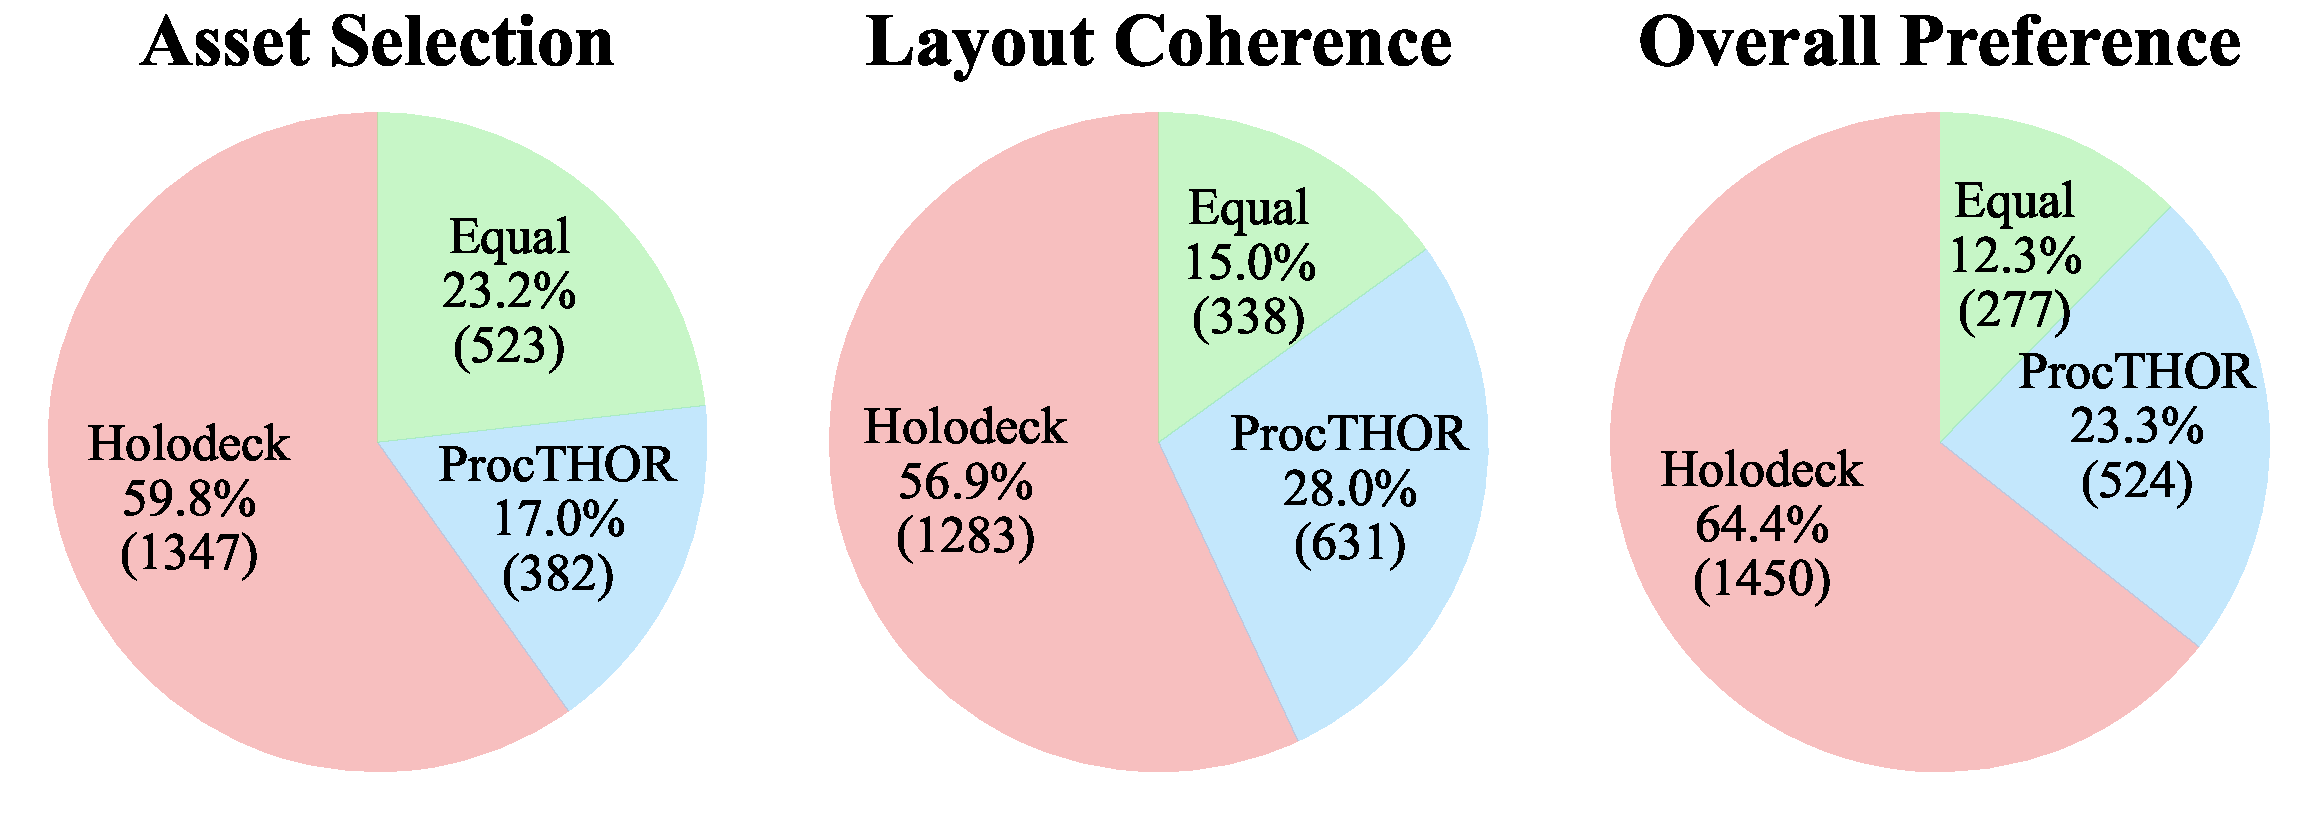
\includegraphics[width=8.3cm]{images/total_pie_plot.pdf}
    \caption{Comparative human evaluation of \holodeck and \procthor across three criteria. The pie charts show the distribution of annotator preferences, showing both the percentage and the actual number of annotations favoring each system.}
    \label{fig: holodeck vs. procthor}
    \vspace{-0.5cm}
\end{figure}

We conduct comprehensive human evaluations to assess the quality of \holodeck scenes, with a total of 680 graduate students participating in three user studies: (1) a comparative analysis on \textbf{residential scenes} with \procthor as the baseline; (2) an examination of \holodeck's ability in generating \textbf{diverse scenes}, and (3) an ablation study to validate the effectiveness of our \textbf{layout design} method. Through these user studies, we demonstrate that \holodeck can create residential scenes of better quality than previous work while being able to extend to a wider diversity of scene types.

\subsection{Comparative Analysis on Residential Scenes} \label{sec: holodeck vs procthor}
This study collects human preference scores to compare \holodeck with \procthor \cite{procthor}, the sole prior work capable of generating complete, interactable scenes. Our comparison focuses on residential scenes, as \procthor is limited to four types: \textit{bathroom}, \textit{bedroom}, \textit{kitchen}, and \textit{living room}.

% This study aims to collect human preference scores between \holodeck and prior work. We compare against \procthor, the only prior work that generates complete and interactable scenes. We compare \holodeck with \procthor on the residential scenes as \procthor supports only supports the following four scene types: 

% beThe closest existing approach for comparison is \procthor~\cite{procthor}, which supports four types of residential scenes .% This user study aims to collect the human preferences over the residential scenes generated by \holodeck and \procthor.
\smallbreak
\noindent \textbf{Setup.} We prepared 120 scenes for human evaluation, comprising 30 scenes per scene type, for both \holodeck and the \procthor baseline. The \procthor baseline has access to the same set of Objaverse assets as \holodeck. For \holodeck, we take the scene type, e.g., ``bedroom'', as the prompt to generate the scenes. We pair scenes of the same scene type from the two systems, resulting in 120 paired scenes for human evaluation. For each paired scene, we display two shuffled top-down view images of the scenes from the two systems.
% \footnote{The order of the two images is randomly shuffled, and the annotator doesn't know which system generates which scene.}
We ask the annotator to choose which scene is better or equally good based on three questions: (1) \textbf{Asset Selection}: which selection of 3D assets is more accurate/faithful to the scene type? (2) \textbf{Layout Coherence}: which arrangement of 3D assets adheres better to realism and common sense (considering the position and orientation)? and (3) \textbf{Overall Preference}: which of the two scenes would you prefer given the scene type? 
\smallbreak
\noindent \textbf{Humans prefer \holodeck over \procthor.}
Figure \ref{fig: holodeck vs. procthor} presents a clear preference for \holodeck in the comparative human evaluation against \procthor, with a majority of annotators favoring \holodeck for Asset Selection (59.8\%), Layout Coherence (56.9\%), and showing a significant preference in Overall Preference (64.4\%).
\begin{figure}[!t]
\centering
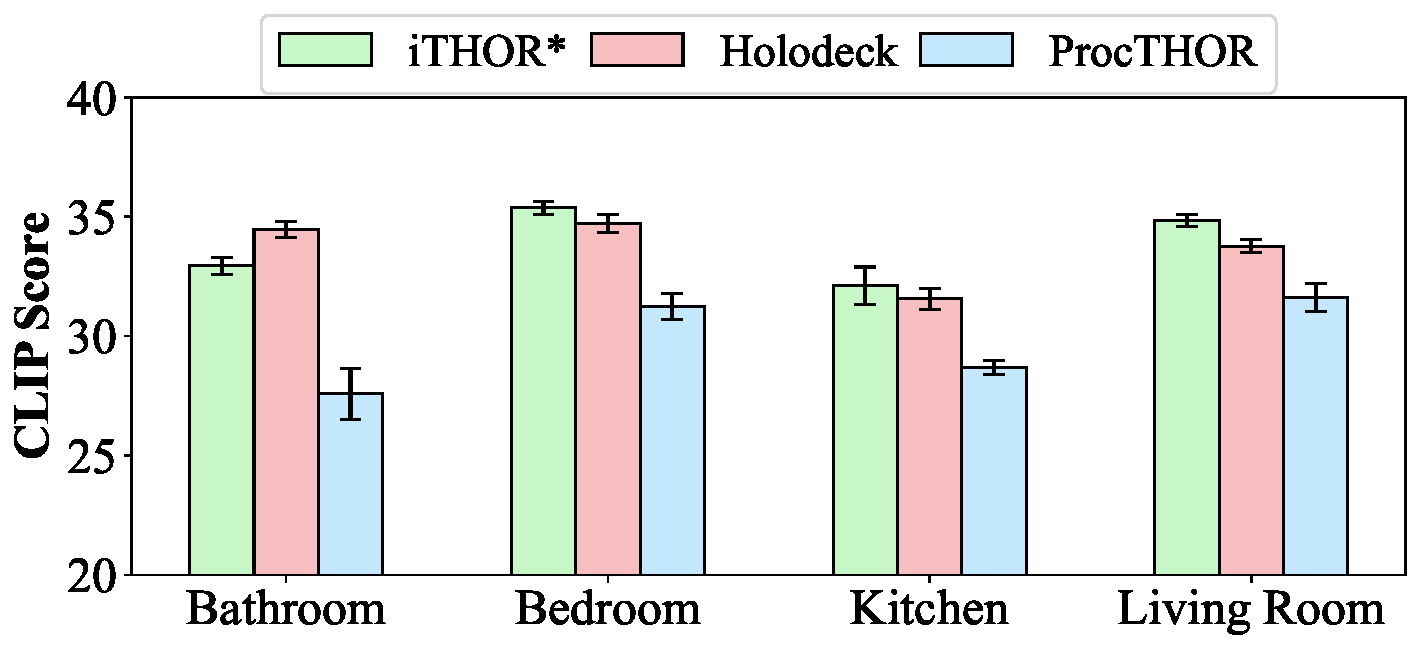
\includegraphics[width=8.3cm]{images/clip_scores_new.pdf}
    \caption{CLIP Score comparison over four residential scene types. * denotes iTHOR scenes are designed by human experts.}
    \label{fig: clip_score}
    \vspace{-0.5cm}
\end{figure}

\begin{figure*}[!t]
\centering
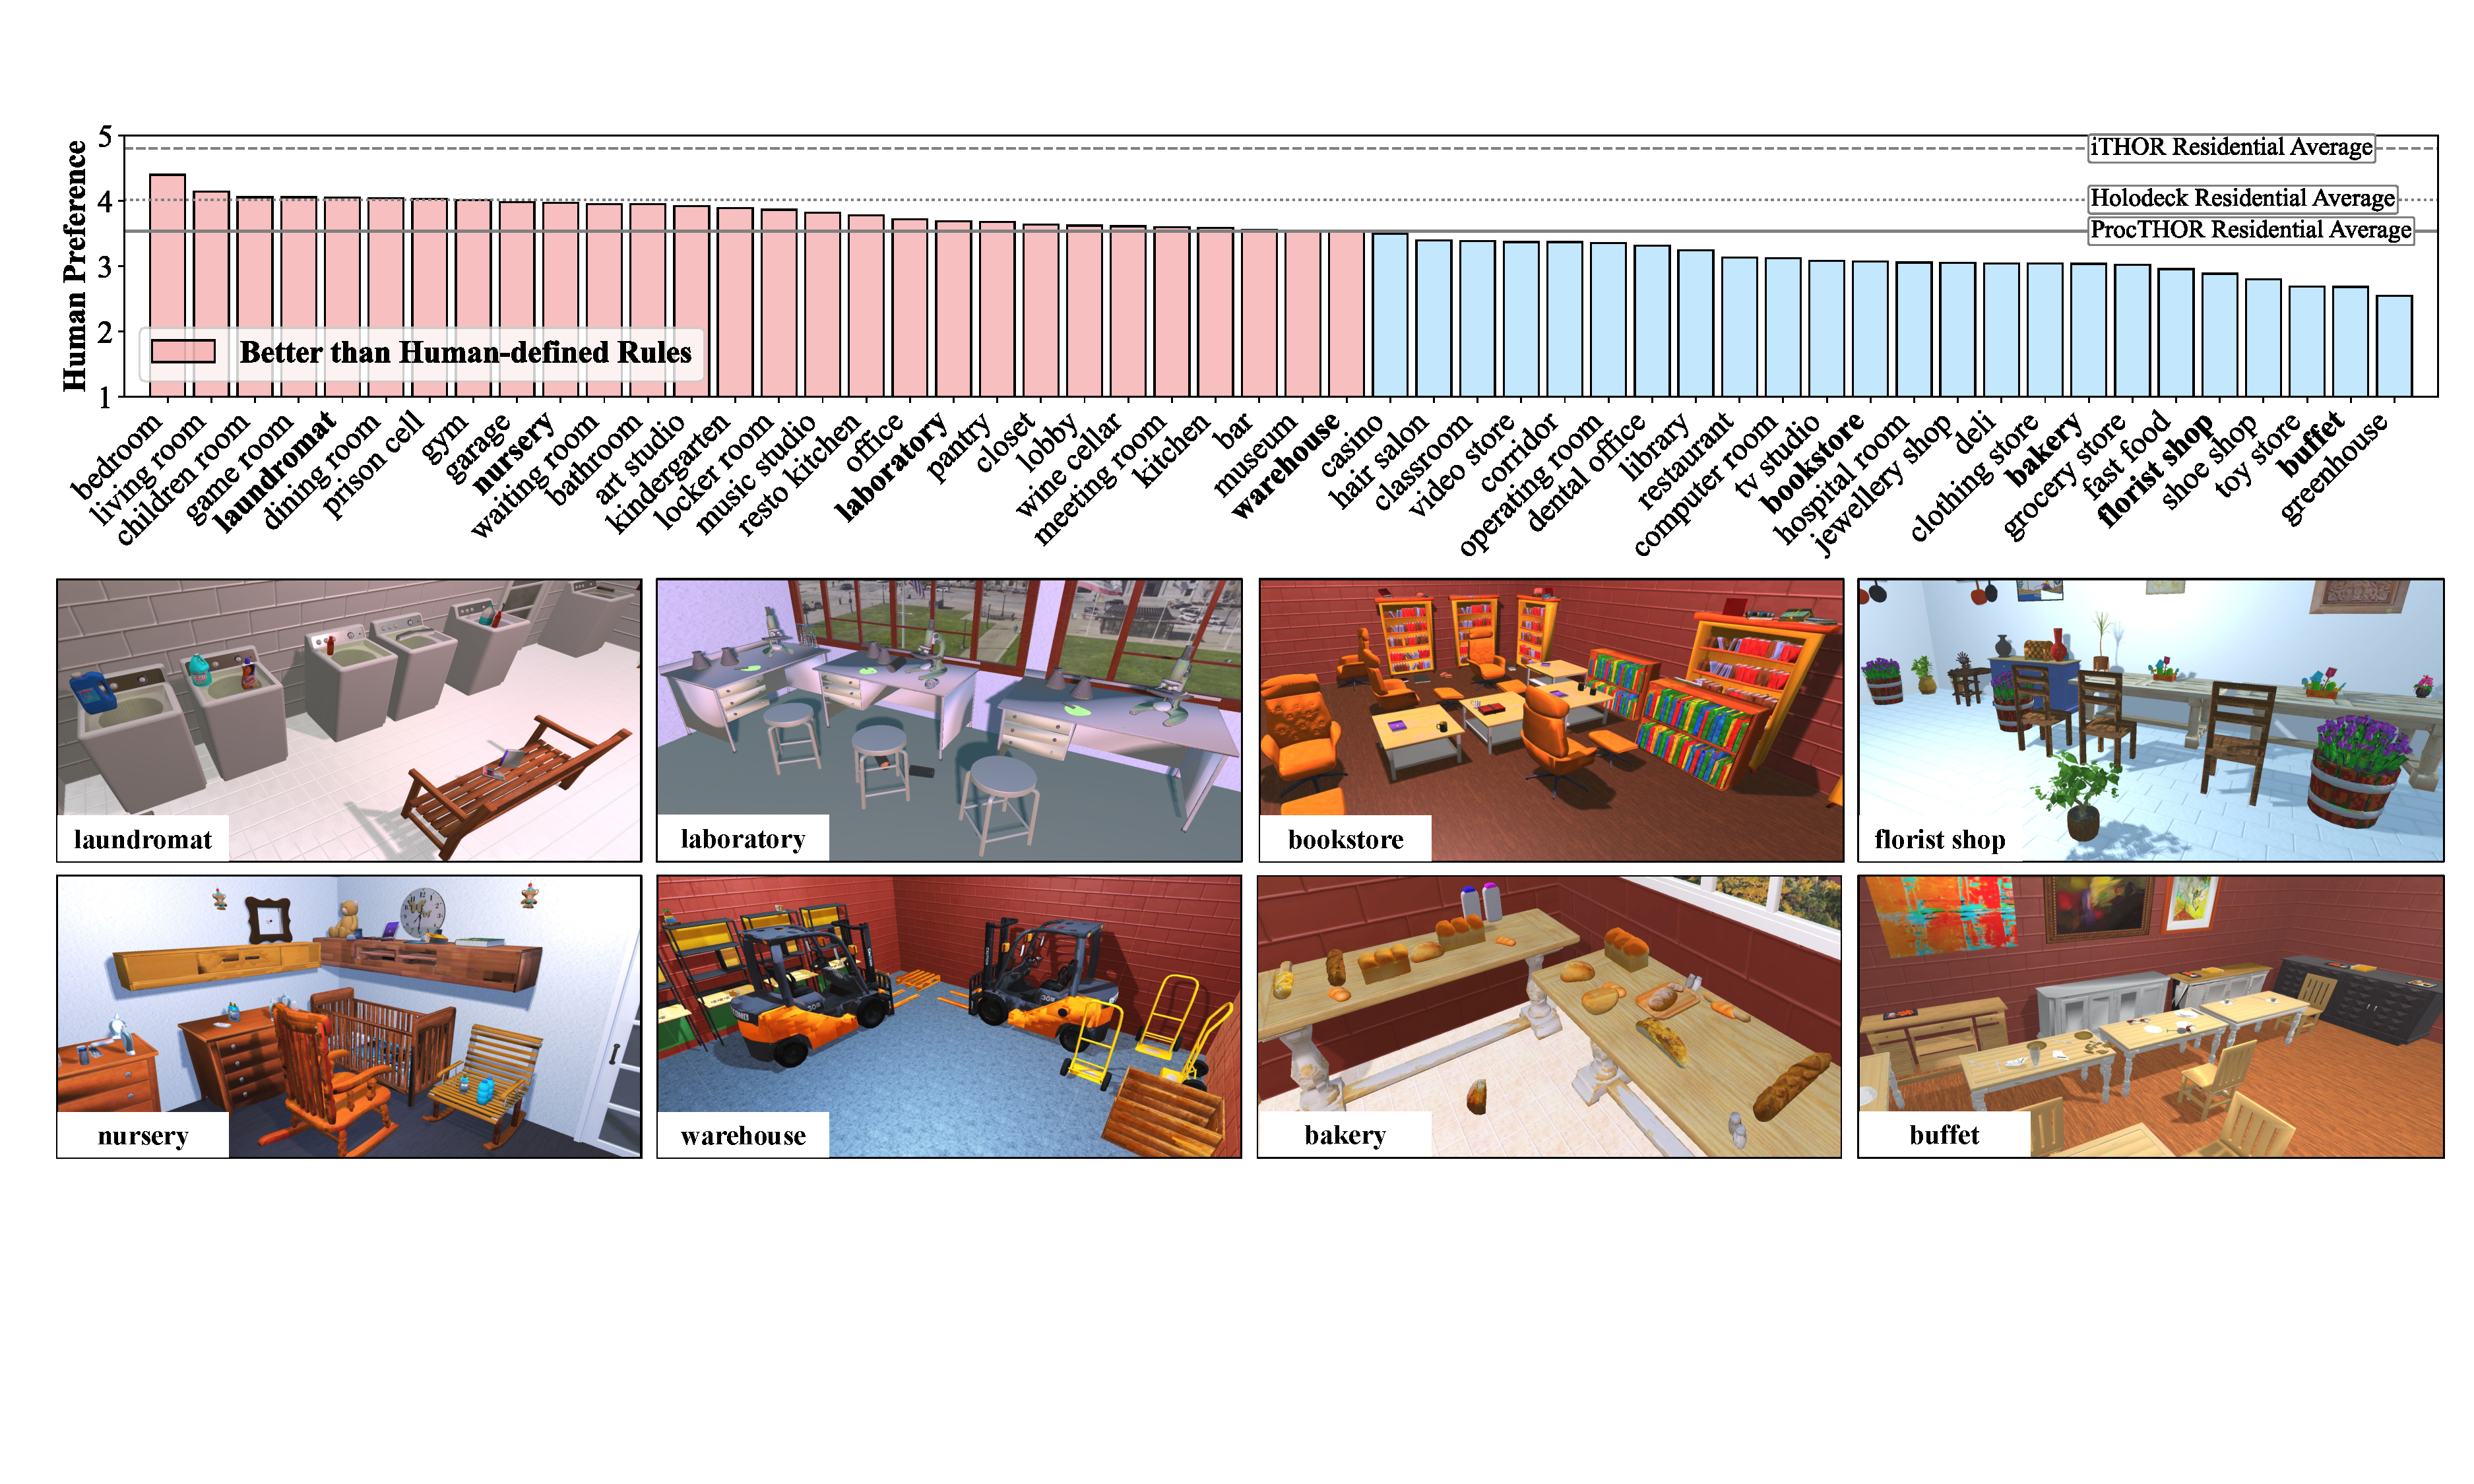
\includegraphics[width=\textwidth]{images/mit_scenes.pdf}
    \caption{Human evaluation on 52 scene types from MIT Scenes \cite{quattoni2009recognizing} with qualitative examples. The three horizontal lines represent the average score of iTHOR, \holodeck, and \procthor on four types of residential scenes (\textit{bedroom}, \textit{living room}, \textit{bathroom} and \textit{kitchen}.)}
    \label{fig: mit scenes}
    \vspace{-0.4cm}
\end{figure*}
In addition to human judgments, we employ CLIP Score\footnote{Here, we use OpenCLIP \cite{ilharco_gabriel_2021_5143773} with ViT-L/14 trained on LAION-2B \cite{schuhmann2022laionb}. We use cosine similarity times 100 as the CLIP Score.} \cite{hessel2021clipscore} to quantify the visual coherence between the top-down view of the scene and its corresponding scene type embedded in a prompt template ``\textit{a top-down view of [scene type]}''. Besides, we add human-designed scenes from iTHOR \cite{ai2thor} as the upper bound for reference. Figure \ref{fig: clip_score} shows the CLIP scores of \holodeck exceed \procthor with great margins and closely approach the performance of iTHOR, demonstrating \holodeck's ability to generate visually coherent scenes faithful to the designated scene types. The CLIP Score experiment agrees with our human evaluation.

\subsection{\textbf{\holodeck} on Diverse Scenes}
To evaluate \holodeck's capability beyond residential scenes, we have humans rate its performance on 52 scene types\footnote{Limited by the \procthor framework, we filter those scenes types that require special structures such as \textit{swimming pool}, \textit{subway}, etc.} from MIT Scenes Dataset~\cite{quattoni2009recognizing}, covering five categories: Stores (\textit{deli}, \textit{bakery}), Home (\textit{bedroom}, \textit{dining room}), Public Spaces (\textit{museum}, \textit{locker room}), Leisure (\textit{gym}, \textit{casino}) and Working Space (\textit{office}, \textit{meeting room}).
\smallbreak
\noindent \textbf{Setup.} We prompt \holodeck to produce five outputs for each type using only the scene name as the input, accumulating 260 examples across the 52 scene types. Annotators are presented with a top-down view image and a 360-degree video for each scene and asked to rate them from 1 to 5 (with higher scores indicating better quality), considering asset selection, layout coherence, and overall match with the scene type. To provide context for these scores, we include residential scenes from \procthor and iTHOR in this study, with 20 scenes from each system.
\smallbreak
\noindent \textbf{\holodeck can generate satisfactory outputs for most scene types.}
Figure~\ref{fig: mit scenes} demonstrates the human preference scores for diverse scenes with qualitative examples. Compared to \procthor's performance in residential scenes, \holodeck achieves higher human preference scores over half of (28 out of 52) the diverse scenes. Given that \procthor relies on human-defined rules and residential scenes are relatively easy to build with common objects and simple layout, \holodeck's breadth of competence highlights its robustness and flexibility in generating various indoor environments. However, we notice that \holodeck struggles with scenes requiring more complex layouts such as \textit{restaurant} or unique assets unavailable in Objaverse, e.g., ``a dental x-ray machine'' for the scene \textit{dental office}.
Future work can improve the system by incorporating more assets and introducing more sophisticated layout algorithms.
\subsection{Ablation Study on Layout Design} \label{sec: layout ablation}
% \begin{table}[!t]
%     \centering
%     \resizebox{8.3cm}{!}{%
%     \begin{tabular}{ccccc}
%     \Xhline{3\arrayrulewidth}  
%      \textbf{Method}    & \textbf{Bathroom} & \textbf{Bedroom} & \textbf{Kitchen} & \textbf{Living Room}\\ \hline
 
%     \textsc{Absolute}   & 0.369 {\footnotesize $\pm$ 0.014} & 0.343 {\footnotesize $\pm$ 0.011} & 0.407 {\footnotesize $\pm$ 0.015} & 0.336 {\footnotesize $\pm$ 0.011} \\
%     \textsc{Random}    & 0.422 {\footnotesize $\pm$ 0.014} & 0.339 {\footnotesize $\pm$ 0.009} & 0.367 {\footnotesize $\pm$ 0.011} & 0.348 {\footnotesize $\pm$ 0.008} \\
%     \textsc{edge}      & 0.596 {\footnotesize $\pm$ 0.018} & 0.657 {\footnotesize $\pm$ 0.016} & \textbf{0.655} {\footnotesize $\pm$ 0.018} & 0.672 {\footnotesize $\pm$ 0.016}  \\\hline
%      \textsc{Constraint}   & \textbf{0.696} {\footnotesize $\pm$ 0.019}& \textbf{0.745} {\footnotesize $\pm$ 0.017} & 0.654 {\footnotesize $\pm$ 0.017} & \textbf{0.728} {\footnotesize $\pm$ 0.017} \\\Xhline{3\arrayrulewidth}
%     \end{tabular} 
%     }
%     \caption{Mean Reciprocal Rank $\uparrow$ (human-ranked) of different object placement methods.}
%     %\textsc{Constraint}: the default method of \holodeck using spatial relational constraints; \textsc{Absolute}: LLM-defined absolute positions; \textsc{Random} and \textsc{Edge}: randomly place the objects or put them at the edge of the room (close to the wall).}
%     \label{tab:placement_abalation}
%     \vspace{-0.5cm}
% \end{table}

\begin{table}[!t]
    \centering
    \resizebox{8.3cm}{!}{%
    \begin{tabular}{cccccc}
    \toprule
     \textbf{Method}    & \textbf{Bathroom} & \textbf{Bedroom} & \textbf{Kitchen} & \textbf{Living Room} & \textbf{Average}\\ 
     \midrule
 
    \textsc{Absolute}   & 0.369 & 0.343 & 0.407  & 0.336  & 0.364\\
    \textsc{Random}    & 0.422 & 0.339  & 0.367  & 0.348  & 0.369\\
    \textsc{edge}      & 0.596  & 0.657  & \textbf{0.655} & 0.672 & 0.645\\
    \midrule
     \textsc{Constraint}   & \textbf{0.696} & \textbf{0.745}  & 0.654  & \textbf{0.728} & \textbf{0.706} \\
     \bottomrule
    \end{tabular} 
    }
    \caption{Mean Reciprocal Rank ($\uparrow$) of different layouts ranked by human. \textsc{Constraint}: using spatial relational constraints; \textsc{Absolute}: LLM-defined absolute positions; \textsc{Random}: randomly place the objects and \textsc{Edge}: put objects at the edge of the room.}
    \label{tab:placement_abalation}
    \vspace{-0.4cm}
\end{table}

This user study aims to validate the effectiveness of \holodeck's constraint-based layout design method.
\smallbreak
\noindent \textbf{Baselines.} We consider four layout design methods: (1) \textsc{Constraint}: the layout design method of \holodeck; (2) \textsc{Absolute}: directly obtaining the absolute coordinates and orientation of each object from LLM akin to LayoutGPT \cite{feng2023layoutgpt}; (3) \textsc{Random}: randomly place all objects in the room without collision; (4) \textsc{Edge}: placed objects along the walls.\looseness=-1
\smallbreak
\noindent \textbf{Setup.} We modify the residential scenes of \holodeck used in \ref{sec: holodeck vs procthor} by altering the layouts using the previously mentioned methods while keeping the objects in the scene identical. We present humans with four shuffled top-down images from each layout strategy and ask them to rank the four layouts considering out-of-boundary, object collision, reachable space, and layout realism.
\smallbreak
\begin{table*}[!t]
\small
\centering
\resizebox{17cm}{!}{%
\begin{tabular}{lcccccccccccc}
\toprule
\textit{}& \multicolumn{2}{c}{\textbf{Office}}   & \multicolumn{2}{c}{\textbf{Daycare}}  & \multicolumn{2}{c}{\textbf{Music Room}}& \multicolumn{2}{c}{\textbf{Gym}}    & \multicolumn{2}{c}{\textbf{Arcade}} & \multicolumn{2}{c}{\textbf{Average}}   \\ 
\cmidrule{2-13}
\multicolumn{1}{l}{\textbf{Method}} & \multicolumn{1}{c}{Success} & \multicolumn{1}{c}{SPL} & \multicolumn{1}{c}{Success} & \multicolumn{1}{c}{SPL} & \multicolumn{1}{c}{Success} & \multicolumn{1}{c}{SPL} & \multicolumn{1}{c}{Success} & \multicolumn{1}{c}{SPL} & \multicolumn{1}{c}{Success} & \multicolumn{1}{c}{SPL} & \multicolumn{1}{c}{Success} & \multicolumn{1}{c}{SPL}\\ 
\midrule
Random & 3.90 & 0.039 & 4.05 & 0.041 & 5.20 & 0.052 & 2.84 & 0.029 & 2.54 & 0.025 & 3.71 & 0.037 \\
\procthor~\cite{procthor} & 8.77 & 0.031 & 2.87 & 0.011 & 6.17 & 0.027 & 0.68 & 0.002 & 2.06 & 0.005 & 4.11 & 0.015  \\
${+}$\textsc{Objaverse} (ours) & 18.42 & 0.068 & 8.99 & 0.061 & 25.69 & 0.157 & \textbf{18.79} & 0.101 & \textbf{13.21} & \textbf{0.076} & 17.02 & 0.093   \\
${+}$\holodeck (ours) & \textbf{25.05} & \textbf{0.127} & \textbf{15.61} & \textbf{0.127} & \textbf{31.08} & \textbf{0.202} & 18.40 & \textbf{0.110} & 11.84 & 0.069 & \textbf{20.40} & \textbf{0.127}
\\ 
\bottomrule
\end{tabular}
}
\caption{Zero-shot ObjectNav on \noveltythor. \procthor is the model pretrained on \textsc{ProcTHOR-10K} \cite{procthor}. ${+}$\textsc{Objaverse} and ${+}$\textsc{Holodeck} stand for models finetuned on the corresponding scenes. We report Success (\%) and Success weighted by Path Length (SPL).}
\label{tab: embodied_results}
\vspace{-0.5cm}
\end{table*}
\begin{figure}[!t]
\centering
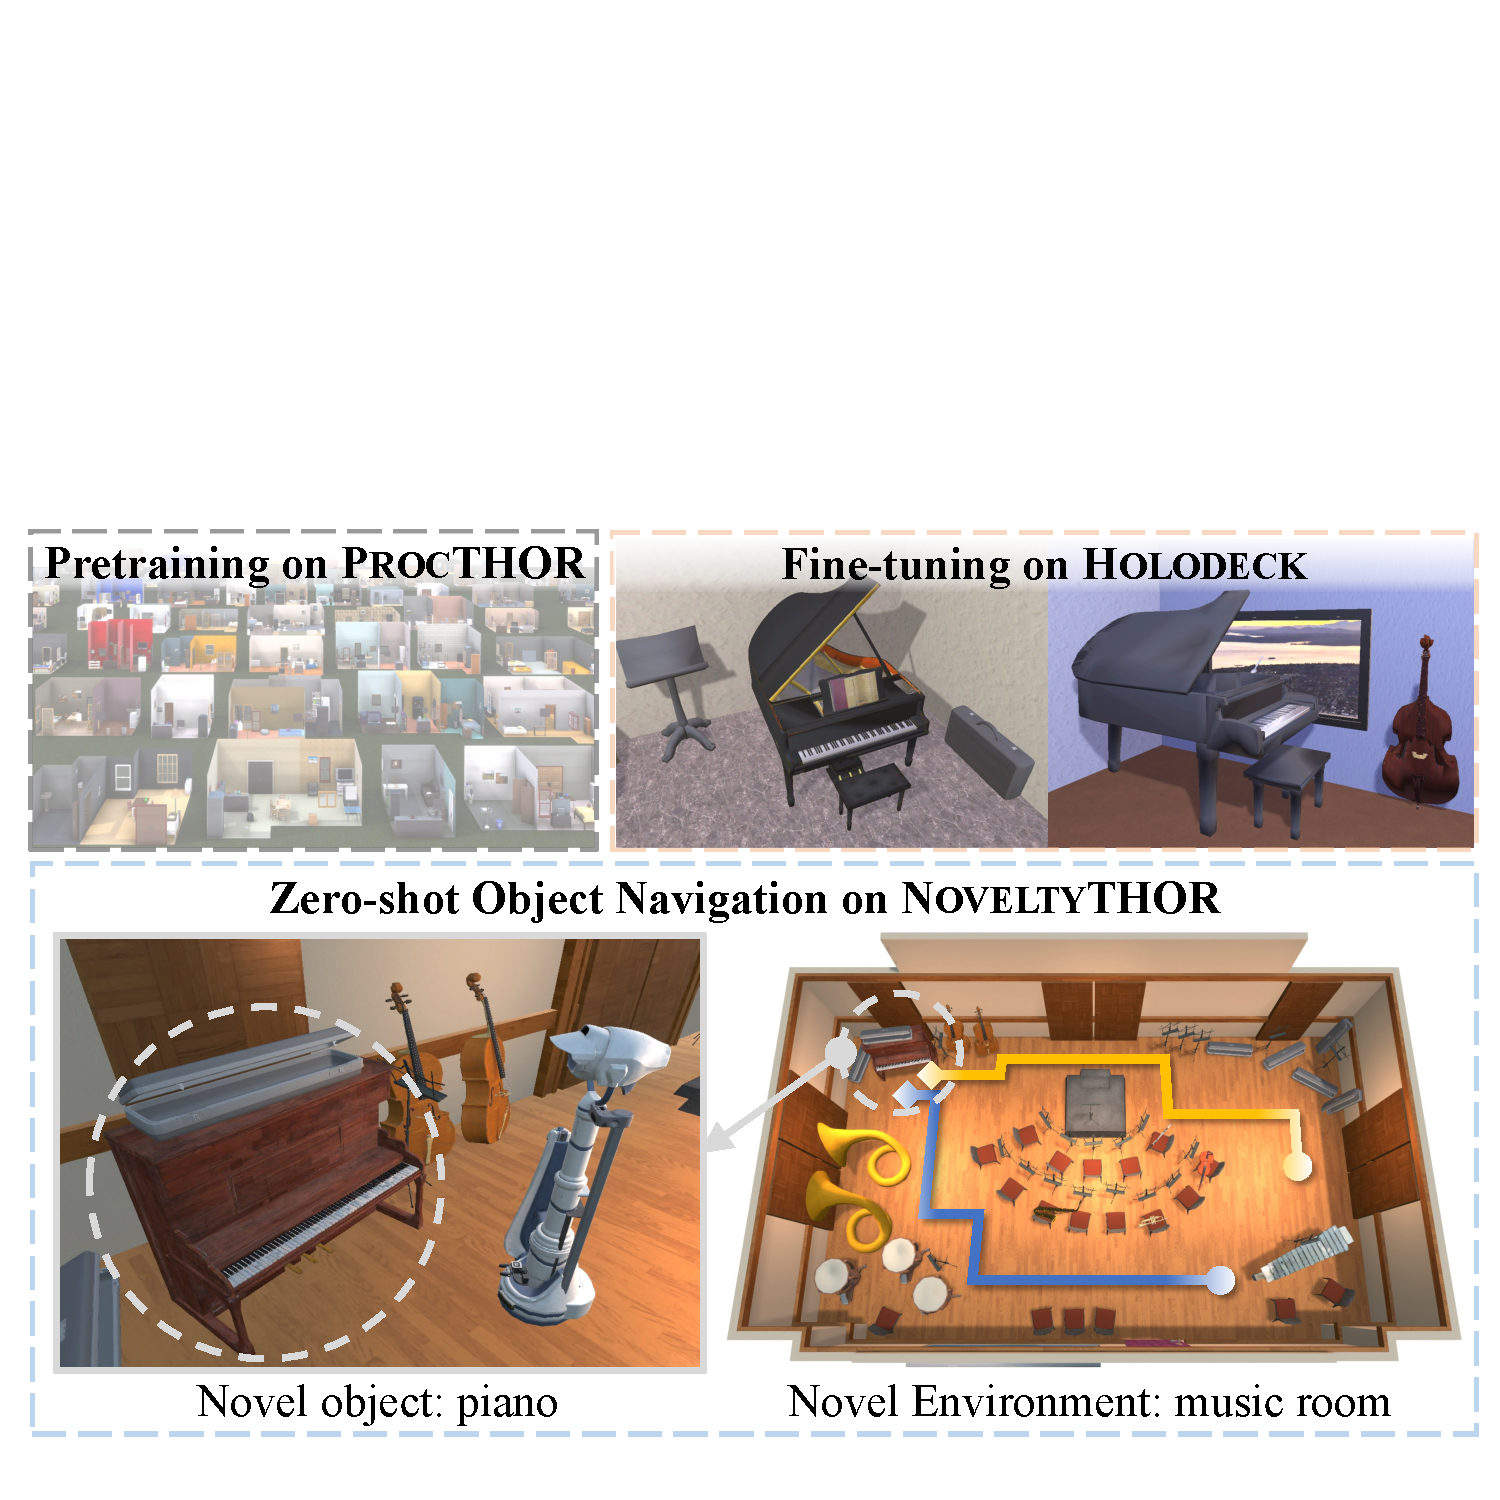
\includegraphics[width=8.3cm]{images/embodied_demo_new.pdf}
    \caption{Zero-shot object navigation in novel scenes. Given a novel scene type, e.g., \textit{Music Room}, \holodeck can synthesize new scenes for fine-tuning to improve the performance of pretrained agents in expert-designed environments.}
    \label{fig: embodied demo}
    \vspace{-0.4cm}
\end{figure}
\noindent \textbf{Constraint-based layout is more reliable.}
Table \ref{tab:placement_abalation} reports the Mean Reciprocal Rank of different layout design methods. \holodeck's constraint-based approach outperforms the other methods significantly on \textit{bathroom}, \textit{bedroom} and \textit{living room}. \textsc{Constraint} and \textsc{Edge} perform similarly on \textit{kitchen}, where it is common to align most objects against walls. The \textsc{Absolute} method performs no better than \textsc{Random} due to its tendency to create scenes with collision and boundary errors (see examples in the supplement), typically rated poorly by humans. These results endorse spatial relational constraints as a viable strategy for generating scenes that adhere to commonsense logic.
